\section{Статистический вес}


Состояние $(\vc{r}, \vc{v}) + (\text{вн. ст. св.})$ формирует элементарную ячейку $d^6 \gamma = d^3 \vc{r} d^3 \vc{v} = dx dy dz \cdot dv_x dv_y dv_z$. Запишем для $N$ частиц произведение $N$ фазовых пространств $$d^{6N} \Gamma = d^6 \gamma_1 \times \dots \times d^6 \gamma_N.$$
Таким образом \textbf{микросостояние} --- точка $\vc{R}^{(6N)} = (\vc{r}_1, \dots, \vc{r}_N, \vc{v}_1. \dots, \vc{v}_N)$ в ФП. Тогда динамика систему $\equiv$ движение точки в ФП. 

Определим \textbf{макросостояние}, как \textit{множество микросостояний (область в ФП), определяемое малым числом параметров}.

Определим \textbf{статистический вес} $\Gamma$, как \textit{число микросостояний, реализующих макросостояние системы (объем области в ФП)}.

\phantom{42}

\boxed{\text{Все доступные микросостояния замкнутой системы равновероятны.}}

\phantom{42}

Тогда \textbf{вероятность} обнаружить систему в некотором состоянии прямо пропорционально его \textit{статическому весу $\Gamma$}. Соответсвенно, состояние \textbf{термодинамического равновесия} --- \textit{состояние с \textbf{максимальным статистическим весом}}. 

Иногда можно свести динамику $N$ частиц, к динамике одной частицы.
Стоит учесть, что частицы независимы (корреляции малы) --- отсутсвуют "коллективные" явления.  

Получим значение для $\Gamma$:
\begin{align*}
    N = \sum\nolimits_{i=1}^M N_i = const, \; \; 
    E = \sum\nolimits_{i=1}^M N_i \varepsilon_i = const.
\end{align*}

Пусть частицы \textbf{различимы}\footnote{
Что применимо к состоянию ядер в кристалле и состоянию электронов в атомах газа.
}, в ячейке любое $N_i$. Тогда получим классическое значение Больцмана, считая $g_i$ --- вероятность нахождения в $i$ ячейке.
\begin{equation}
\boxed{
    \Gamma = \frac{N!}{N_1! N_2! \dots N_M!} \cdot g_1^{N_1} \cdot g_2^{N_2} \cdot \dots \cdot g_M^{N_M} \approx \prod\nolimits_{i=1}^M \lr{\frac{
    g_i N
    }{
    N_i
    }}^{N_i}
}
\end{equation}

Пусть частицы \textbf{нераличимы}\footnote{
Например, атомы идеального газа. Также в приближении Стирлинга похоже на $\Gamma$ для бозонов.} (фермионы). Есть фермионы -- верен "запрет Паули", есть бозоны, для которых нет запрета. Считая, что на уровне $g_i$ ячеек:

$ \Gamma_i = {g_i \cdot (g_i - 1)\cdot (g_i - 2) \cdot \dots \cdot (g_i - N_i + 1)}/{N_i!} =  g_i! / N_i! / (g_i - N_i)!$.

Учитывая, что $g_i \gg N_i$, получим\footnote{
Забавный факт: $\Gamma_{\text{разл}} = N! \cdot \Gamma_{\text{неразл}}$.
}
\begin{equation}
\boxed{
    \Gamma \approx \frac{g_1^{N_1} \cdot g_2^{N_2} \cdot ... \cdot g_M^{N_M}}{N_1! \cdot N_2! \cdot ... \cdot N_M!}
    \approx \exp{\lr{N}} \cdot \prod\nolimits_{i=1}^{M} \lr{\frac{g_i}{N_i}}^{N_i}
}.
\end{equation}

\subsection{Энтропия}
Дабы уйти от гнёта больших чисел перейдём к:
$$\widetilde{S} = \ln \Gamma = - \sum\nolimits_{i=1}^{M} N_i \lr{\ln \frac{N_i}{g_i} - 1}.$$

\subsection{Распределение Гиббса-Больцмана}
Продифференцируем происходящее. $dN = \sum dN_i = 0$, $dE = d(\sum \varepsilon_i N_i) = \sum \varepsilon_i dN_i = 0$, $d\widetilde{S} = - \sum \ln \frac{N_1}{g_i} dN_i = 0$.

Всё это можно взять с произвольными коэффициентами, сложить и вынести $dN_i$:
$$
\sum\nolimits_{i=1}^{M} \lr{
\lambda + \beta \varepsilon_i - \ln \frac{N_i}{g_i}
} dN_i = 0
$$
Тогда 
\begin{equation}
    \boxed{
    N_i = const \cdot g_i \cdot \exp{\lr{- \frac{\varepsilon}{kT}}}
    }, \text{ или\footnote{
    для идеальных систем
    } } \boxed{
    \omega (\varepsilon) = \frac{1}{Z} \cdot g_k \cdot \exp \lr{-\frac{\varepsilon}{kT}}
    }
\end{equation}

где используется нормировочный множитель $Z = \sum_i g_i \exp{\lr{- \frac{\varepsilon_i}{kT}}}$ --- \textbf{статсумма}, $g_k$--- статвес уровня.

\begin{law}[Теплота]
Изменение энергии за счёт перераспределения частиц по состояниям (ячейкам фазового пространства).
\end{law}

Тогда для энтропии верно, что (\textbf{ДОПИСАТЬ/ДОДЕЛАТЬ})
$$
d \widetilde{S} = - \lambda \sum dN_i + \sum \beta \varepsilon_i dN_i = \beta dE = \beta \delta Q = \frac{\delta Q}{kT}, \text{ или } \boxed{S = k \ln \Gamma} .
$$

Стоит заметить, что \textbf{статсумма}:
$$
Z(T, V) = \sum\nolimits_{\text{эн}} g_k \exp{-\frac{\varepsilon_k}{kT}} = \sum\nolimits_{\text{сост}} \exp - \frac{\varepsilon_i}{kT}
$$

Далее см. \textbf{пример №1}. Получаем:
\begin{equation}
\label{energy}
    \boxed{ \phantom{4}
    \overline{\varepsilon}(T) = \lr{
    i_{\text{пост}} + 
    i_{\text{вращ}} + 
    2 i_{\text{кол}}
    } \cdot \frac{1}{2} kT \phantom{4}
    }.
\end{equation}

Есть жесткие молекулы, для них всё знаем в "линейном" и "нелинейном" случае. 

\subsection{Квантовая теплоемкость}
\begin{figure}[h]
    \centering
    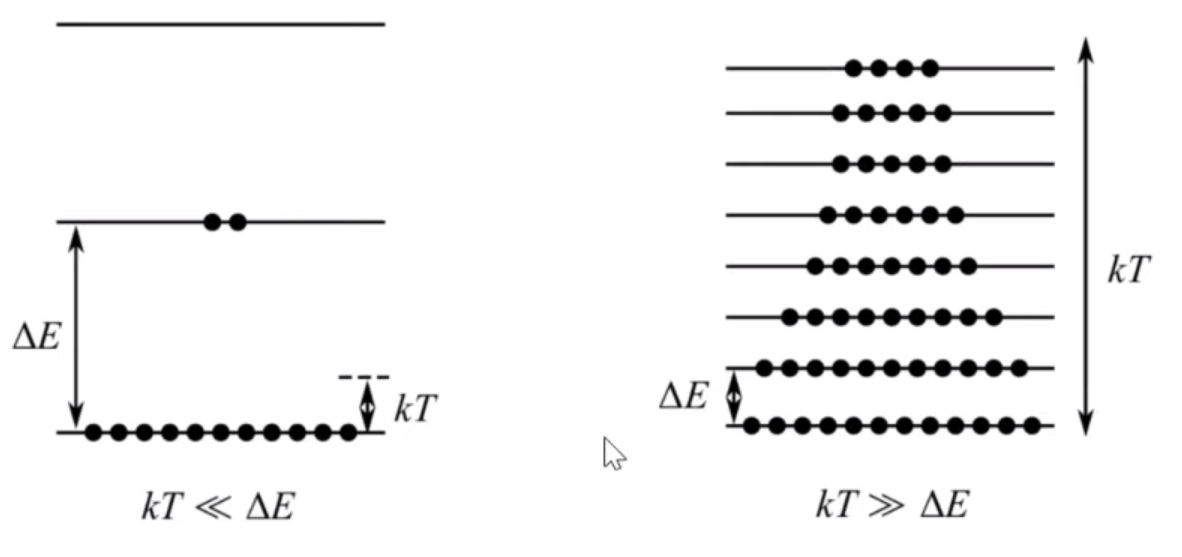
\includegraphics[width=0.4\textwidth]{img_and_tables/quant_c.png}
    \caption{Замороженная vs. полностью возбужденная степень свободы}
    \label{ZvsF}
\end{figure}

\noindent
Для\footnote{
Важно: $\hbar = 1.05 \cdot 10^{-34}$ Дж $\cdot$ с.
} \textbf{вращения} запишем, что
$$\varepsilon_l = \frac{\hbar^2}{2I} l (l + 1), \; \; g_l = 2 l + 1, \; \; l = 0, 1, \dots, \infty.$$
Для \textbf{гармонических колебаний}:
$$
\varepsilon_n = \hbar \omega \lr{n + \frac{1}{2}}, \; \; g_n = 1, \; \; n = 0, 1, \dots, \infty.
$$

Введем \textbf{характеристическую температуру}
$$
\theta = \frac{\Delta E}{k}, \; \; \; \; \;
\theta_{\text{вращ}} = \frac{\hbar}{k I} \sim \frac{1}{mr^2}, \; \; \; \; \;
\theta_{\text{кол}} = \frac{\hbar \omega}{k} \sim \sqrt{\frac{\kappa}{m}}.
$$
